\section{Zemax 制造工程实践}

\subsection{Zemax 公差分析：从设计到可制造}

\englishtitle{Tolerance Analysis for Manufacturing}
\begin{frame}{为什么需要公差分析？}
    \begin{columns}[T]
        \begin{column}{.52\textwidth}
            \begin{block}{现实问题}
                \alert{名义设计}(Nominal Design)在公差为零的理想条件下优化——但真实制造中每个参数都有公差。不加公差分析的设计等于\alert{纸上谈兵}。
            \end{block}

            \bigbreak
            \textbf{公差分析的目的：}
            \begin{enumerate}
                \item 评估制造误差对\alert{最终性能}的影响
                \item 识别\alert{敏感参数}——哪些公差最关键
                \item 在性能与\alert{制造成本}之间找到平衡
                \item 生成\alert{ISO 10110} 图纸的公差规范
            \end{enumerate}
        \end{column}
        \hfill
        \begin{column}{.48\textwidth}
            \begin{block}{没有公差分析的风险}
                \begin{itemize}
                    \item "名义设计很好，实物很差"
                    \item 关键面公差太紧 $\rightarrow$ 成本暴涨
                    \item 非关键面公差太松 $\rightarrow$ 良率过低
                    \item 无法判断量产风险
                \end{itemize}
            \end{block}

            \bigbreak
            \alert{核心原则：}最终交付前必须做公差分析，否则无法评估量产风险。
        \end{column}
    \end{columns}
\end{frame}

\englishtitle{Tolerance Types in Zemax}
\begin{frame}{Zemax 公差操作数类型}
    公差数据编辑器 (Tolerance Data Editor) 中主要有以下公差操作数：

    \begin{table}
        \centering
        \small
        \setlength{\tabcolsep}{3pt}
        \begin{tabular}{p{2cm}|p{3.5cm}|p{5cm}}
            \toprule
            \textbf{类别} & \textbf{操作数} & \textbf{含义} \\
            \midrule
            \multirow{2}{*}{曲率/厚度} & \textbf{TEDR} & 透镜中心厚度公差 \\
            & \textbf{TEPR} & 曲率半径公差(以光圈数表示) \\
            \midrule
            \multirow{3}{*}{偏心/倾斜} & \textbf{TSDX / TSDY} & 透镜表面 X/Y 方向偏心 \\
            & \textbf{TSTX / TSTY} & 透镜表面绕 X/Y 轴倾斜 \\
            & \textbf{TEDX / TEDY} & 透镜整体 X/Y 方向偏心 \\
            \midrule
            \multirow{2}{*}{不规则度} & \textbf{TIRR} & 表面不规则度(球面) \\
            & \textbf{TIRX / TIRY} & 表面不规则度(柱面/非球面) \\
            \midrule
            折射率/阿贝数 & \textbf{TIND / TABB} & 折射率 / 阿贝数公差 \\
            \midrule
            装调补偿器 & \textbf{COMP} & 后焦距、空气间隔补偿 \\
            \bottomrule
        \end{tabular}
        \caption{Zemax 主要公差操作数分类}
        \label{tab:tolerance_operands}
    \end{table}
\end{frame}

\englishtitle{Compensators and Tolerance Wizard}
\begin{frame}{补偿器与公差向导}
    \begin{columns}[T]
        \begin{column}{.52\textwidth}
            \textbf{补偿器 (Compensator)：}
            在公差分析中，某些参数可以在装配时\alert{主动调整}以补偿制造误差：

            \begin{itemize}
                \item \textbf{后焦距}(Back Focus)— 最常用补偿器
                \item \textbf{空气间隔}— 双胶合或镜组间距
                \item \textbf{像面位置}— 传感器/底片平面
                \item \textbf{镜组整体位移}— 调整整组位置
            \end{itemize}

            \bigbreak
            \alert{补偿器模拟了实际装配中的调校自由度。}
        \end{column}
        \hfill
        \begin{column}{.48\textwidth}
            \textbf{公差向导 (Tolerance Wizard)：}

            Zemax 提供预设的公差模板：
            \begin{itemize}
                \item \textbf{Optimax} — 精密光学加工
                \item \textbf{Edmund Optics} — 标准商业级
                \item \textbf{Asphericon} — 非球面专用
                \item \textbf{自定义} — 按供应商实际能力设置
            \end{itemize}

            \bigbreak
            向导自动生成 TSDX/TSDY/TIRR/TEDR 等全套操作数，只需选择预设等级即可。
        \end{column}
    \end{columns}
\end{frame}

\englishtitle{Sensitivity Analysis and Monte Carlo}
\begin{frame}{逆灵敏度分析与蒙特卡洛模拟}
    \begin{columns}[T]
        \begin{column}{.55\textwidth}
            \textbf{步骤一：逆灵敏度分析 (Inverse Sensitivity)}
            \begin{itemize}
                \item 设定设计指标(如 RMS 弥散斑 $< 3\,\mu\text{m}$)
                \item ZEMAX \alert{反算每个参数允许的最大公差}
                \item 每次计算仅考虑\alert{一个公差}
                \item 输出结果：每个面的公差容限表
                \item 识别最敏感面：\alert{光线折射越大的面，公差越紧}
            \end{itemize}

            \bigbreak
            \textbf{关键洞察：}
            如果最紧公差的透镜是\alert{平凸透镜}(加工难度低)，则即使公差比常规精度小，仍然可实现。
        \end{column}
        \hfill
        \begin{column}{.45\textwidth}
            \textbf{步骤二：蒙特卡洛 (Monte Carlo)}
            \begin{itemize}
                \item 将所有公差\alert{一起}计算
                \item 在每个公差范围内随机取值
                \item 生成大量"虚拟样品"
                \item 统计弥散斑尺寸的概率分布
            \end{itemize}

            \begin{block}{判定准则}
                \alert{若 $>50\%$ 概率满足设计指标}\\
                $\Longrightarrow$ 该公差范围可接受\\
                $\Longrightarrow$ 加工后仍满足设计要求
            \end{block}
        \end{column}
    \end{columns}
\end{frame}


\englishtitle{Practical Tolerance Guidelines}
\begin{frame}{实用公差参考值}
    \begin{table}
        \centering
        \small
        \setlength{\tabcolsep}{3pt}
        \begin{tabular}{p{2.8cm}|p{2.5cm}|p{2.5cm}|p{2.5cm}}
            \toprule
            \textbf{公差项} & \textbf{精密级} & \textbf{标准级} & \textbf{商业级} \\
            \midrule
            曲率半径(光圈) & $\le 1$ fringe & $1\sim 3$ fringes & $3\sim 5$ fringes \\
            中心厚度 (mm)     & $\pm 0.01$ & $\pm 0.03$ & $\pm 0.05\sim 0.10$ \\
            表面偏心 (mm)     & $\le 0.005$ & $\le 0.015$ & $\le 0.03$ \\
            表面倾斜 (arcmin) & $\le 0.5$ & $\le 1.0$ & $\le 2.0$ \\
            不规则度 (fringe) & $\le 0.25$ & $\le 0.5$ & $\le 1.0$ \\
            折射率             & $\pm 0.0001$ & $\pm 0.0003$ & $\pm 0.0005\sim 0.001$ \\
            阿贝数 (\%)        & $\pm 0.2$ & $\pm 0.5$ & $\pm 0.8$ \\
            \bottomrule
        \end{tabular}
        \caption{不同等级的光学制造公差参考值}
        \label{tab:tolerance_guidelines}
    \end{table}

    \alert{注意：}具体公差值取决于镜头用途、供应商能力和成本预算。上述为一般参考，实际应以供应商的具体能力为准。
\end{frame}

\subsection{玻璃替换：材料优化策略}

\englishtitle{Glass Substitution — Motivation and Concept}
\begin{frame}{为什么需要玻璃替换？}
    \begin{columns}[T]
        \begin{column}{.50\textwidth}
            \textbf{传统玻璃选择方法的困境：}

            \begin{block}{Conrady d-D 与模型玻璃}
                \begin{enumerate}
                    \item \textbf{Conrady d-D}：仅追迹少数波长，缩放后优化使差异为零——仅适用于可见光简化
                    \item \textbf{模型玻璃 (Model Glass)}：用 $n$, $\nu$, 部分色散偏离三个参数理想化色散，作为连续变量优化
                \end{enumerate}
            \end{block}

            \begin{alertblock}{模型玻璃的致命缺陷}
                \begin{itemize}
                    \item 获得好方案后必须\alert{将模型玻璃转换为真实玻璃}
                    \item 转换后用新玻璃重新优化，性能\alert{反而比模型方案更差}
                    \item 真实玻璃的最优设计可能\alert{结构形式完全不同}
                    \item 整个过程需要\alert{两次优化}，结果不可预测
                \end{itemize}
            \end{alertblock}
        \end{column}
        \hfill
        \begin{column}{.50\textwidth}
            \begin{block}{玻璃替换方法 — 解决一切问题}
                \begin{itemize}
                    \item 在优化中\alert{直接使用真实玻璃目录}
                    \item 无需"模型 $\to$ 真实"的二次转换
                    \item 全局优化自动迭代替换，找到\alert{真正最优}的真实玻璃
                    \item 支持所有商用目录：Schott, Hoya, Ohara, CDGM 等
                \end{itemize}
            \end{block}

            \bigbreak
            \begin{center}
                \fbox{\textbf{1. 设 Substitute solve} $\to$ \textbf{2. 建评价函数} $\to$ \textbf{3. Hammer 优化} $\to$ \textbf{4. 筛选结果}}
            \end{center}

            \alert{结论：}玻璃替换是 OpticStudio 中\alert{最有效}的玻璃选择方法——直接使用真实玻璃，全程可控。
        \end{column}
    \end{columns}
\end{frame}

\englishtitle{Step 1 — Set Substitute Solve in LDE}
\begin{frame}{Step 1：在 LDE 中设置 Substitute 求解类型}
    \begin{columns}[T]
        \begin{column}{.42\textwidth}
            以系统自带的 \alert{Doublet.zmx} 为例(位于 \texttt{\{Zemax\}/Samples/Sequential/Objectives/})：

            \begin{enumerate}
                \item 打开示例文件
                \item 在 LDE 中\alert{双击(或右键单击)玻璃参数}
                \item 在 Solve 对话框中将 Type 设为 \alert{"Substitute"}
                \item 字母 \alert{"S"} 出现在玻璃后——表示已启用替换
            \end{enumerate}

            \bigbreak
            \textbf{可选操作：}
            \begin{itemize}
                \item 在 Solve 对话框的 Catalog 字段中输入目录名(如 "Hoya")，限制替换范围到\alert{单一供应商}
            \end{itemize}
        \end{column}
        \hfill
        \begin{column}{.58\textwidth}
            \begin{figure}
                \centering
                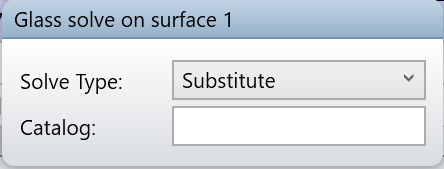
\includegraphics[width=0.95\textwidth]{Figure/玻璃替换/Picture1zh-cn.png}
                \caption{在 LDE 中将玻璃的 Solve 类型设为 Substitute}
                \label{fig:glass_step1}
            \end{figure}
        \end{column}
    \end{columns}
\end{frame}

\englishtitle{Step 2 — Build Merit Function}
\begin{frame}{Step 2：构建 RMS 波前默认评价函数}
    \begin{columns}[T]
        \begin{column}{.42\textwidth}
            \begin{enumerate}
                \item 打开 \texttt{Optimize $\rightarrow$ Merit Function Editor}
                \item 使用 \alert{RMS $\rightarrow$ Wavefront} 默认评价函数
                \item 可根据需要添加自定义操作数(如焦距、像高约束)
                \item \alert{建议使用 RMS + 波前}：对大多数系统效果最好
            \end{enumerate}

            \bigbreak
            \textbf{为什么选 RMS Wavefront？}
            \begin{itemize}
                \item 直接对应波像差，与瑞利判据和 Strehl 比关联
                \item 对色差敏感——玻璃替换的本质就是优化色散匹配
            \end{itemize}
        \end{column}
        \hfill
        \begin{column}{.58\textwidth}
            \begin{figure}
                \centering
                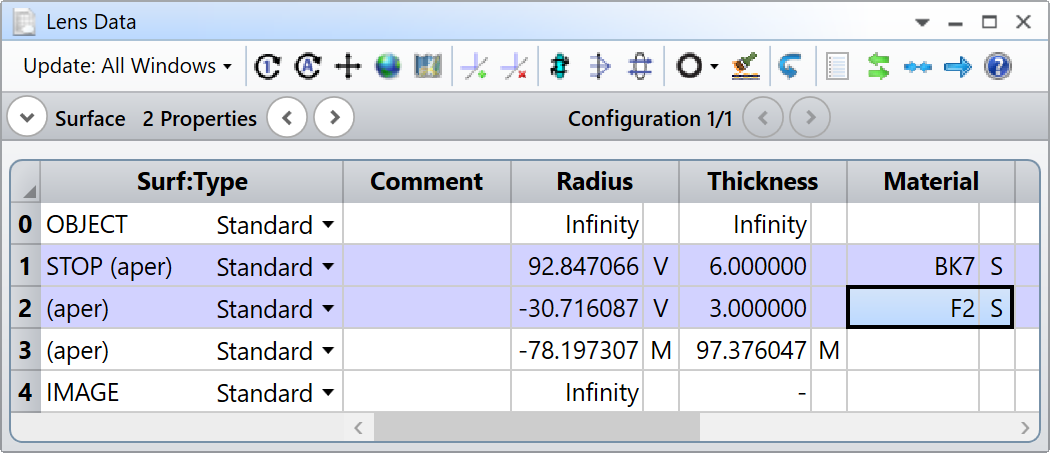
\includegraphics[width=0.95\textwidth]{Figure/玻璃替换/Picture2zh-cn.png}
                \caption{构建 RMS Wavefront 默认评价函数}
                \label{fig:glass_step2}
            \end{figure}
        \end{column}
    \end{columns}
\end{frame}

\englishtitle{Step 3 — Hammer Optimization}
\begin{frame}{Step 3：Hammer 全局优化 + OPD 实时观察}
    \begin{columns}[T]
        \begin{column}{.60\textwidth}
            \begin{enumerate}
                \item 使用 \texttt{Optimize $\rightarrow$ Hammer Current}
                \item \alert{不能用 Local Optimization！}
                \begin{itemize}
                    \item 玻璃替换导致评价函数\alert{不连续跳跃}
                    \item 局部优化无法处理离散的玻璃变化
                \end{itemize}
                \item 启用 \alert{"Auto Update"}——实时观察 LDE 中玻璃的动态替换
                \item 假设使用 Schott 目录，OPD 从初始约 0.5 逐步降低
            \end{enumerate}

            \bigbreak
            \textbf{优化过程中你会看到：}
            \begin{itemize}
                \item LDE 中的玻璃型号\alert{在变化}
                \item OPD 曲线\alert{逐步下降}
                \item Hammer 自动尝试成千上万种玻璃组合
            \end{itemize}
        \end{column}
        \smallbreak
        \begin{column}{.40\textwidth}
            \begin{figure}
                \centering
                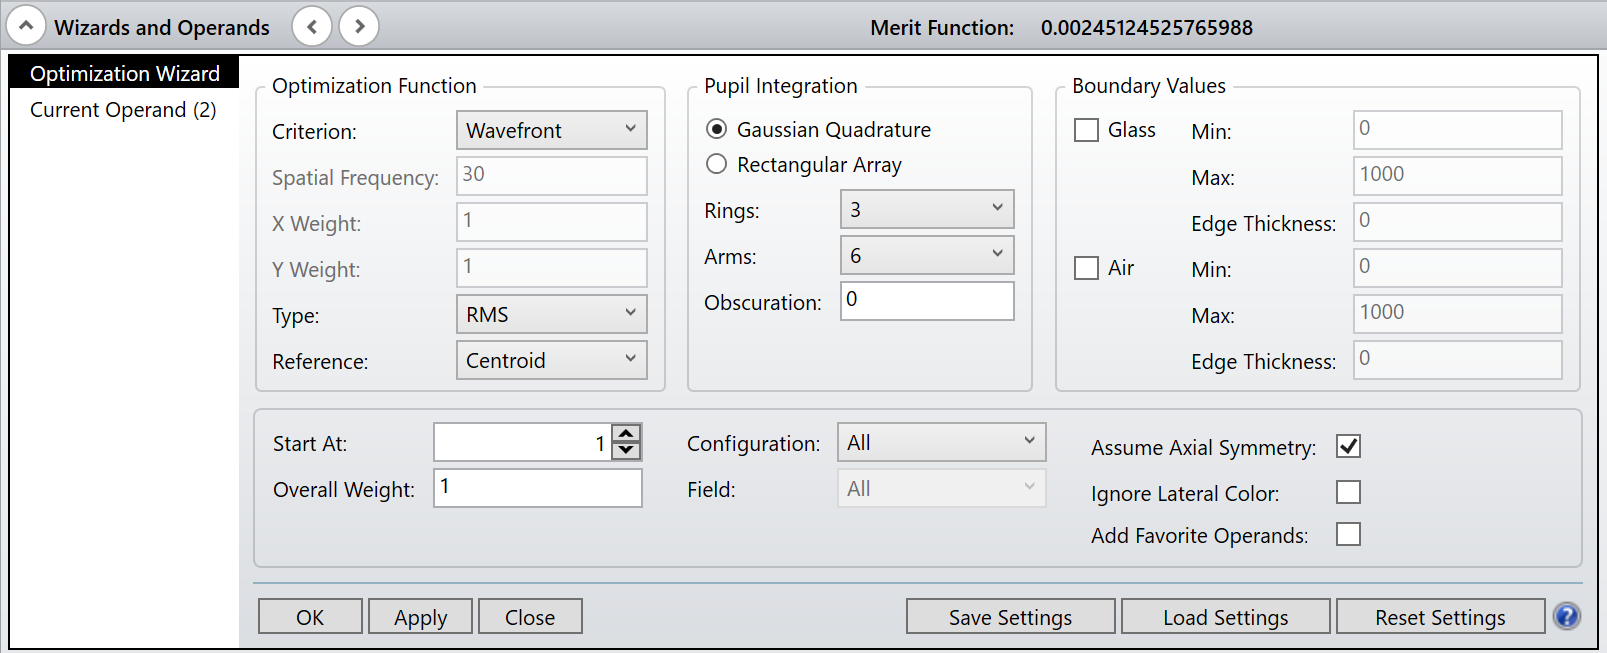
\includegraphics[width=0.95\textwidth]{Figure/玻璃替换/Picture3zh-cn.png}
                \caption{Hammer 优化——玻璃替换自动运行}
                \label{fig:glass_step3a}
            \end{figure}
            \smallbreak
            \begin{figure}
                \centering
                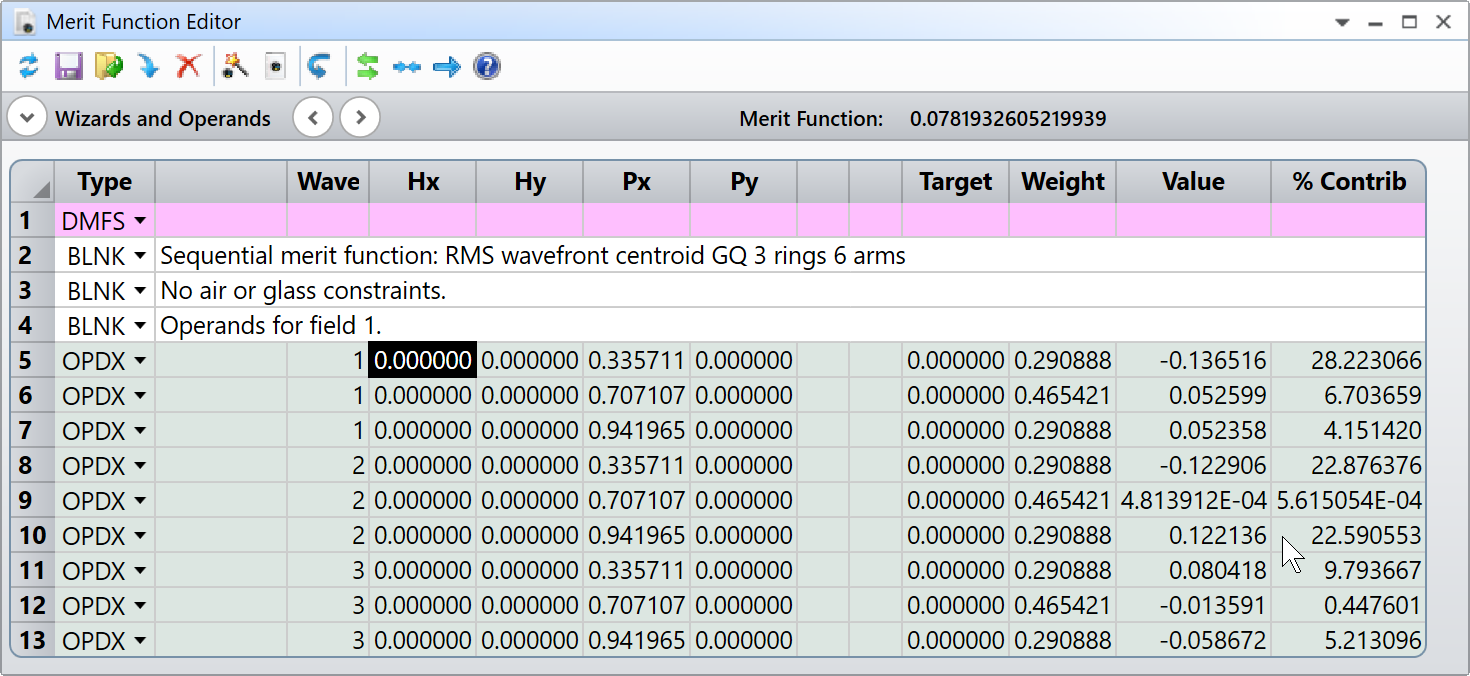
\includegraphics[width=0.95\textwidth]{Figure/玻璃替换/Picture4zh-cn.png}
                \caption{OPD 优化前 vs 优化后对比——显著改善}
                \label{fig:glass_step3b}
            \end{figure}
        \end{column}
    \end{columns}
\end{frame}

\englishtitle{Step 4 — Restrict Glass Catalogs}
\begin{frame}{Step 4：限制玻璃目录范围}
    \begin{columns}[T]
        \begin{column}{.60\textwidth}
            \textbf{两种限制方式：}
            \begin{enumerate}
                \item \textbf{全局限制}：
                \texttt{System Explorer $\to$ Materials Catalogs}，只勾选需要的目录
                \item \textbf{单玻璃限制}：
                在 Glass Solve 的 Catalog 字段输入特定目录名
            \end{enumerate}

            \bigbreak
            常用目录：Schott, Hoya, Ohara, \alert{CDGM(成都光明)}, Sumita
        \end{column}
        \hfill
        \begin{column}{.40\textwidth}
            \begin{figure}
                \centering
                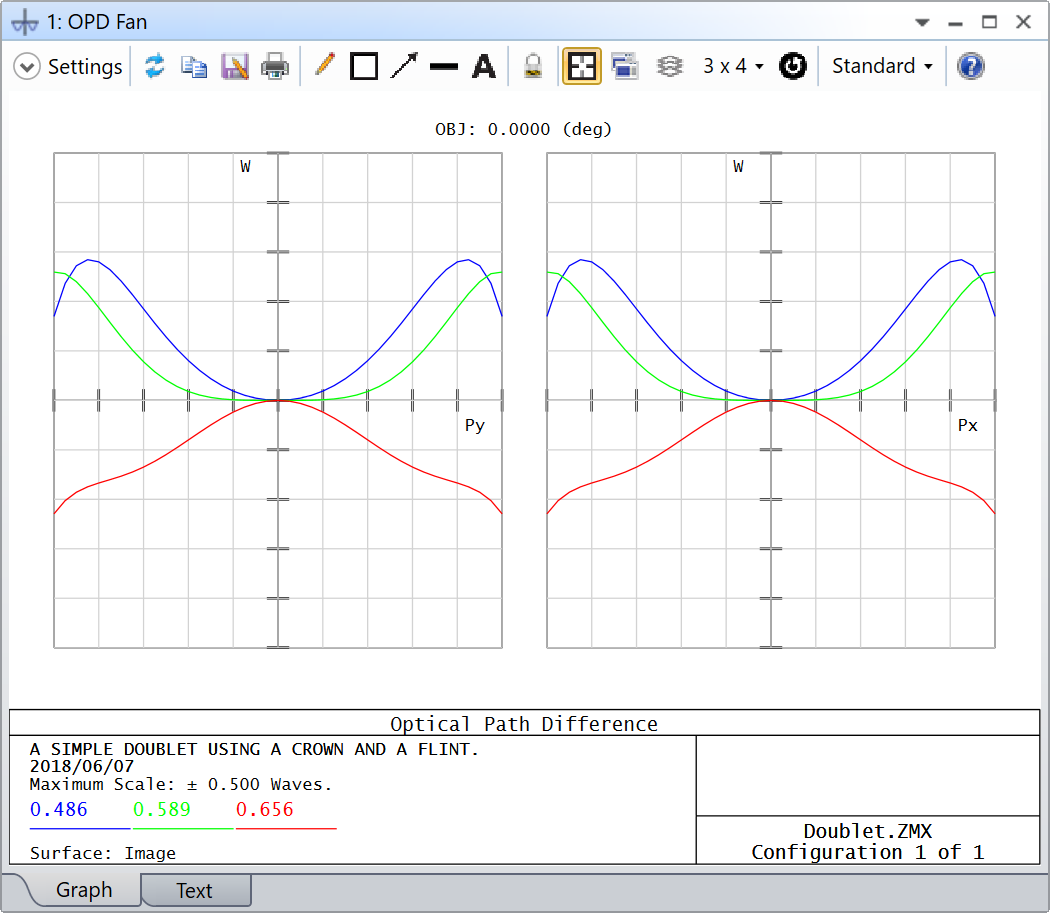
\includegraphics[width=\textwidth]{Figure/玻璃替换/Picture6zh-cn.png}
                \caption{单玻璃 Solve 限制到 Hoya 目录后的 LDE}
                \label{fig:glass_step4b}
            \end{figure}
        \end{column}
    \end{columns}
\end{frame}

\englishtitle{Glass Substitution Template — Filter by Cost and Durability}
\begin{frame}{玻璃替换模板：按成本与耐候性进一步筛选}
    \begin{columns}[T]
        \begin{column}{.65\textwidth}
            \textbf{打开模板：}
            \texttt{Libraries $\rightarrow$ Glass Substitution Template}

            \smallbreak
            勾选 \alert{Use Glass Substitution Template} 后可过滤：
            \begin{enumerate}
                \item \textbf{Status(状态)}
                \begin{itemize}
                    \item \alert{Preferred} — 推荐！低成本、最稳定
                    \item Standard / Special / Obsolete / Melt
                \end{itemize}
                \item \textbf{Relative Cost} — 以 N-BK7 为基准
                \item \textbf{耐候性/化学稳定性} — 耐候、耐污、耐酸、耐碱、耐磷酸盐
            \end{enumerate}

            \bigbreak
            \begin{block}{最佳实践}
                \alert{始终勾选 "Preferred" 状态} \\
                确保使用成本最低、供应最充足、化学最稳定的玻璃。
            \end{block}
        \end{column}
        \hfill
        \begin{column}{.35\textwidth}
            \begin{figure}
                \centering
                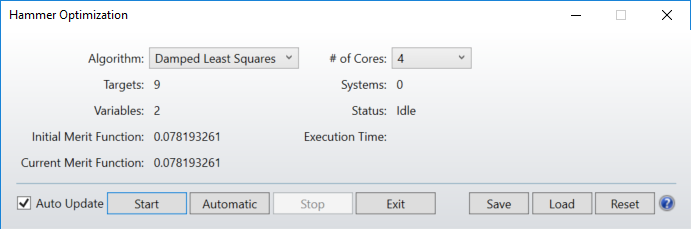
\includegraphics[width=\textwidth]{Figure/玻璃替换/Picture7zh-cn.png}
                \caption{菜单：打开 Glass Substitution Template}
                \label{fig:glass_tpl_menu}
            \end{figure}
            \hfil
            \begin{figure}
                \centering
                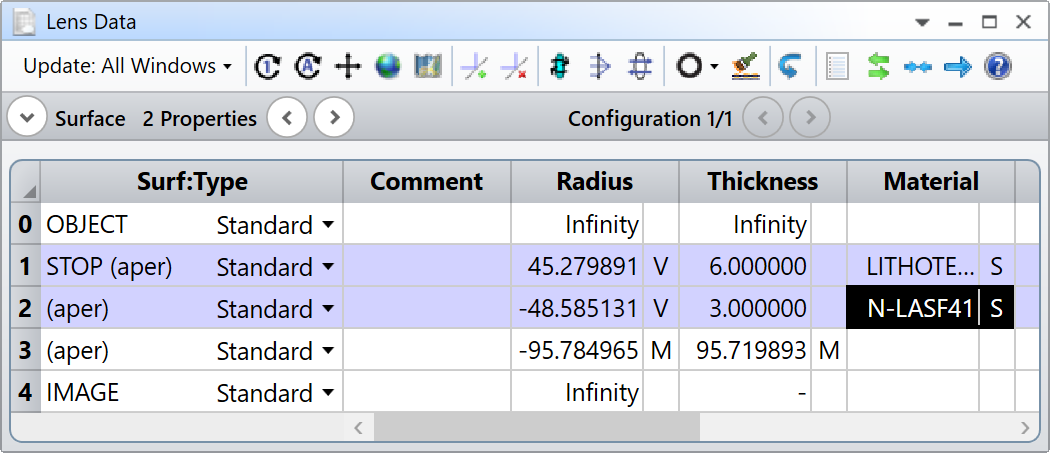
\includegraphics[width=\textwidth]{Figure/玻璃替换/Picture8zh-cn.png}
                \caption{玻璃替换模板——按 Status/Cost/耐候性过滤}
                \label{fig:glass_tpl_interface}
            \end{figure}
        \end{column}
    \end{columns}
\end{frame}

% \englishtitle{Glass Catalog Status and Material Browser}
% \begin{frame}{玻璃目录与材质浏览器}
%     \begin{columns}[T]
%         \begin{column}{.65\textwidth}
%             在 \texttt{Libraries $\rightarrow$ Materials Catalog} 中查看完整玻璃目录：

%             \begin{itemize}
%                 \item 每行玻璃有 \alert{Status 字段}明确标注
%                 \item Preferred(首选)玻璃通常是 N-BK7 及其等效品
%                 \item Standard / Special 玻璃按需使用
%                 \item Obsolete 玻璃\alert{不应用于新设计}
%             \end{itemize}

%             \bigbreak
%             \textbf{Status 字段含义速查：}
%             \begin{table}
%                 \centering
%                 \footnotesize
%                 \begin{tabular}{l|l}
%                     \toprule
%                     Preferred & 推荐！低成本、稳定、供应充足 \\
%                     Standard  & 可用但非首选的常规玻璃 \\
%                     Special   & 特殊玻璃，需确认可用性 \\
%                     Obsolete  & \alert{已淘汰}，不推荐新设计使用 \\
%                     Melt      & 定制熔炼，交期长、成本高 \\
%                     \bottomrule
%                 \end{tabular}
%             \end{table}
%         \end{column}
%         \hfill
%         \begin{column}{.35\textwidth}
%             \begin{figure}
%                 \centering
%                 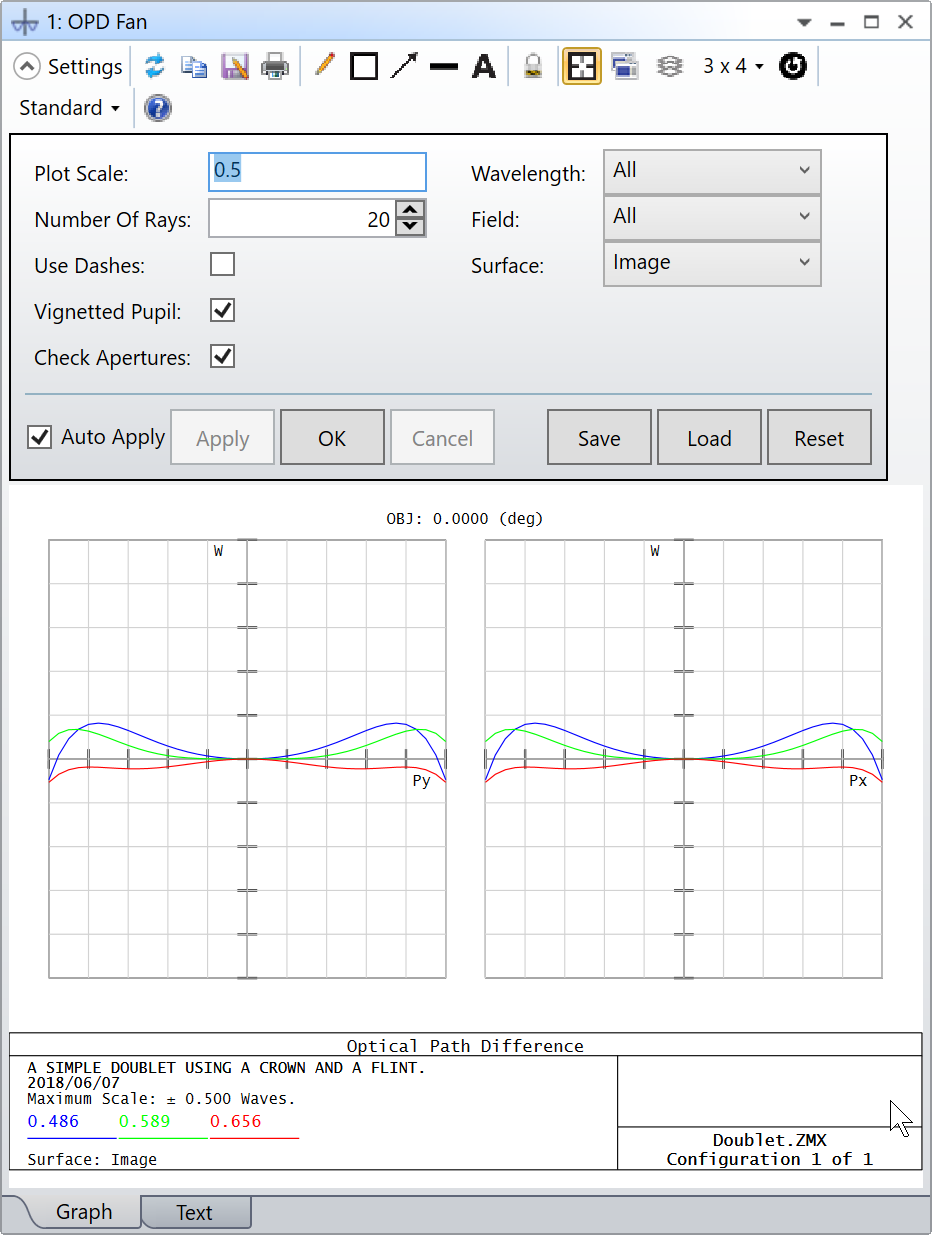
\includegraphics[width=0.9\textwidth]{Figure/玻璃替换/Picture9zh-cn.png}
%                 \caption{玻璃目录中的 Status 字段说明}
%                 \label{fig:glass_catalog_status}
%             \end{figure}
%         \end{column}
%     \end{columns}
% \end{frame}

\englishtitle{Automation — ZPL and ZOS-API}
\begin{frame}{自动化：ZPL 宏与 ZOS-API}
    \begin{columns}[T]
        \begin{column}{.60\textwidth}
            \textbf{ZPL 宏 (Zemax Programming Language)：}
            \begin{itemize}
                \item 编写 ZPL 脚本在 OpticStudio 内部\alert{批量执行}玻璃替换
                \item 适用于：大量设计变体的自动化探索
                \item 可在脚本中设置玻璃目录、替换范围、评价函数
            \end{itemize}

            \bigbreak
            \textbf{ZOS-API (Zemax OpticStudio API)：}
            \begin{itemize}
                \item 通过 \alert{MATLAB、Python、C\#} 等外部语言控制
                \item 适用于：集成到自动化优化流水线
                \item 可与其他工程软件(如结构分析、热分析)联动
            \end{itemize}
        \end{column}
        \hfill
        \begin{column}{.40\textwidth}
            \begin{figure}
                \centering
                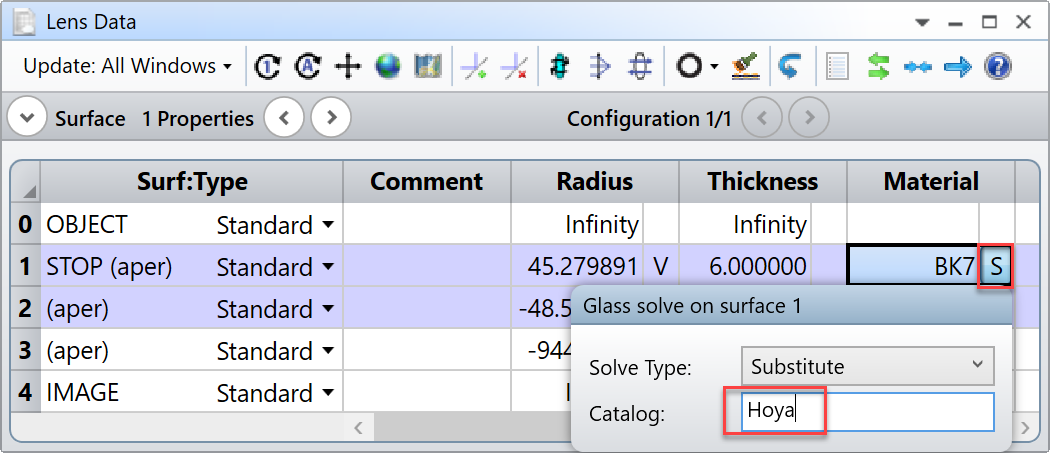
\includegraphics[width=0.9\textwidth]{Figure/玻璃替换/Picture11zh-cn.png}
                \caption{ZPL 宏实现自动化玻璃替换}
                \label{fig:zpl_glass_sub}
            \end{figure}
        \end{column}
    \end{columns}
\end{frame}

\subsection{从设计到制造：集成工作流}

\englishtitle{Design-to-Manufacturing Workflow}
\begin{frame}{从设计到制造的完整流程}
    \begin{figure}
        \centering
        \fbox{\textbf{初始设计}}\hspace{0.5em}
        $\longrightarrow$\hspace{0.5em}
        \fbox{\textbf{玻璃替换}}\hspace{0.5em}
        $\longrightarrow$\hspace{0.5em}
        \fbox{\textbf{名义优化}}\hspace{0.5em}
        $\longrightarrow$\hspace{0.5em}
        \fbox{\textbf{公差分析}}\hspace{0.5em}
        $\longrightarrow$\hspace{0.5em}
        \fbox{\textbf{迭代}}\hspace{0.5em}
        $\longrightarrow$\hspace{0.5em}
        \fbox{\textbf{ISO 图纸}}

        \bigbreak
        \renewcommand{\arraystretch}{1.8}
        \begin{tabular}{p{3cm}|p{4cm}|p{4cm}}
            \toprule
            \textbf{阶段} & \textbf{关键操作} & \textbf{工具/方法} \\
            \midrule
            1. 初始设计  & 定义规格、选择初始结构   & System Explorer, LDE \\
            2. 玻璃替换  & Substitute solve, Hammer & 全局优化 + 玻璃模板 \\
            3. 名义优化  & 以像质为目标精细优化      & Local + Hammer 优化 \\
            4. 公差分析  & 灵敏度 + 蒙特卡洛        & Tolerance Wizard, TOLR \\
            5. 迭代优化  & 修改敏感面/调整公差      & 回到步骤 2 或 3 \\
            6. ISO 图纸  & 输出制造公差规范         & ISO 10110 标准 \\
            \bottomrule
        \end{tabular}
        \caption{从设计到制造的完整工作流}
        \label{tab:design_to_manufacturing_workflow}
    \end{figure}

    \alert{理解要点：}玻璃替换和公差分析不是独立的——它们共同确保设计在\alert{可用的真实材料}和\alert{可实现的制造公差}下达到目标性能。
\end{frame}

\englishtitle{Key Takeaways for Manufacturing}
\begin{frame}{制造工程实践要点总结}
    \begin{columns}[T]
        \begin{column}{.50\textwidth}
            \textbf{公差分析要点：}
            \begin{enumerate}
                \item 名义优化只是\alert{第一步}——不加公差分析等于纸上谈兵
                \item 使用\alert{公差向导}选择供应商预设等级
                \item \alert{补偿器}模拟装配调校自由度——必须设置
                \item 灵敏度分析找出\alert{关键参数}——这些是成本驱动因素
                \item 蒙特卡洛 $\ge 1000$ 样本评估\alert{统计良率}
                \item TOLR 操作数可\alert{在优化中直接降低}公差灵敏度
                \item 最终输出 ISO 10110 制造图纸
            \end{enumerate}
        \end{column}
        \hfill
        \begin{column}{.50\textwidth}
            \textbf{玻璃替换要点：}
            \begin{enumerate}
                \item 设置 Solve 为 \alert{"Substitute"}
                \item 使用\alert{全局优化}(Hammer/Global Search)
                \item 勾选玻璃替换模板的\alert{Preferred} 状态
                \item 按\alert{成本和耐候性}进一步筛选
                \item 匹配\alert{供应商目录}(Schott/Hoya/CDGM 等)
                \item 模型玻璃方法已过时——\alert{直接使用真实玻璃}
            \end{enumerate}

            \bigbreak
            \begin{block}{设计的终点是制造}
                \centering
                \alert{名义设计好 $\neq$ 能做出来}\\
                玻璃选得好 $\rightarrow$ 公差给得对 $\rightarrow$ 良率达标\\
                $\Longrightarrow$ 这才是真正的"设计完成"
            \end{block}
        \end{column}
    \end{columns}
\end{frame}

\englishtitle{Integration with Previous Chapters — Complete Picture}
\begin{frame}{全流程整合：从理论到制造}
    \begin{alertblock}{五步学习路径回顾}
        \begin{enumerate}
            \item \textbf{像差理论基础(Ch.1)}：波像差、PSF、OTF —— 理解"什么是好"
            \item \textbf{横向像差图分析(Ch.2)}：Ray Fan 诊断各像差 —— 理解"哪里不好"
            \item \textbf{Zemax 设计实践(Ch.3)}：操作数、评价函数、优化流程 —— 学会"怎么优化"
            \item \textbf{机器视觉工程(Ch.4)}：Edmund Optics 视角 —— 理解"工程权衡"
            \item \textbf{制造工程实践(Ch.5)}：公差分析 + 玻璃替换 —— 实现"能做出来"
        \end{enumerate}
    \end{alertblock}

    \bigbreak
    \begin{center}
        \textbf{理论 $\rightarrow$ 诊断 $\rightarrow$ 优化 $\rightarrow$ 权衡 $\rightarrow$ \alert{制造}}
    \end{center}

    \bigbreak
    镜头设计的终极目标不是"名义性能最优的数字文件"，而是\alert{能以合理成本批量生产且性能稳定的物理镜头}。
\end{frame}
